\chapter{Aξιολόγηση Συστήματος}\label{ch:evaluation}

\section{Κοινωνικός Αποκλεισμός και Επανένταξη Εικονικών Οντοτήτων}
Αρχικά παρουσιάζουμε μία εικόνα επίτευξης του στόχου αυτής της διπλωματικής εργασίας. Είναι ένα δίκτυο στο οποία αλλάζει η συμπεριφορά των εικονικών οντοτήτων και παρόλ'αυτά οι κακόβουλες αποκλείονται ενώ οι καλόβουλες προτιμώνται για τις υπηρεσίες.

\diagramscale{Κοινωνικός Αποκλεισμός και Επανένταξη Εικονικών Οντοτήτων}{dynamicoscilate.png}{0.3}

Στην πρώτη εικόνα είναι το αρχικό δίκτυο όπου η κάθε Ε.Ο. έχει τυχαίους φίλους. Δίπλα μπορούμε να δούμε πώς ισορροπεί μετά από μερικά βήματα ενώ στην τρίτη εικόνα φαίνεται πώς αμέσως μετά από μία αλλαγή συμπεριφοράς οι νέες κακόβουλες οντότητες έχουν πολλά βέλη πάνω τους. Στην τετάρτη εικόνα βλέπουμε πώς οι οντότητες αποκλείονται μόλις εντοπιστούν από τις υπόλοιπες ενώ στις άλλες 2 μπορούμε να δούμε την επανένταξή τους όταν γίνουν και πάλι καλές.
\newpage
\section{Μέση Ικανοποίηση Εικονικών Οντοτήτων στο RT-IOT}

Για να μπορέσει να παρουσιαστεί η αξία του RT-IOT διεξήχθησαν διαφορών τύπων προσομοιώσεις ώστε να μπορέσουν να εξαχθούν τα κατάλληλα συμπεράσματα. Αρχικά αναλύθηκε η συμπεριφορά του RT-IOT ως σύστημα για να φανεί η επίδοση του σε σε σταθερά και δυναμικά περιβάλλοντα. Έτσι συνδυάσαμε 3 διαφορετικές και ανεξάρτητες μεταξύ τους καταστάσεις για να δούμε συνολικά 8 πιθανές καταστάσεις του συστήματος. Όλες οι τιμές είναι ο μέσος όρος τον τιμών από 30-50 διαφορετικά δίκτυα όπου οι παράμετροι είναι ίδιοι.

Οι 3 καταστάσεις ήταν:
\begin{enumerate}
\item \textbf{Collusion (col):} Όταν είναι ενεργή αυτή η κατάσταση οι κακόβουλες εικονικές οντότητες βρίσκουν άλλες κακόβουλες και τις προωθούν μέσω του συστήματος φήμης.

\item\textbf{Οscillating(osc):} Όταν είναι ενεργή αυτή η κατάσταση η συμπεριφορά των κόμβων που παρέχουν τη υπηρεσία αλλάζει δυναμικά από κακόβουλη σε καλόβουλη διατηρώντας όμως το ποσοστό τον κακόβουλων οντοτήτων σταθερό στο σύστημα.

\item\textbf{Dynamic(dyn):} Όταν είναι ενεργή αυτή η κατάσταση κάποιες Εικονικές Οντότητες παύουν την λειτουργία τους για σύντομο χρονικό διάστημα προσομοιώνοντας την αποσύνδεση μίας συσκευής από το σύστημα.
\end{enumerate}
Στον παρακάτω πίνακα \ref{tab:avg_sat} μπορεί να φανεί το πώς εξελίσσεται το ποσοστό της μέσης ικανοποίησης των εικονικών οντοτήτων στις διαφορές καταστάσεις ανάλογα με το ποσοστό των κακόβουλων Ε.Ο. στο σύστημα


Τα συμπεράσματα που βγαίνουν είναι τα εξής:

\begin{itemize}

\item Σε ένα σταθερό σύστημα το RT-IOT μπορεί να παρέχει άριστου επιπέδου ασφάλεια. Ακόμα και σε δίκτυο με 90\% κακόβουλες Εικονικές Οντότητες η ικανοποίηση είναι  πάνω από 96\%

\item Σε δίκτυο με φυσιολογικό ποσοστό κακόβουλων οντοτήτων (30\% και κάτω) το σύστημα καταφέρνει να παρέχει ικανοποίηση πάνω από 90 \% ακόμα και σε δυναμικά δίκτυα με συνεργαζόμενες κακόβουλες οντότητες όπου αλλάζουν συμπεριφορά (col+osc+dyn)

\item Ακόμα και όταν η ικανοποίηση είναι χαμηλή (κάτω απο 50\%), η ύπαρξη του συστήματος παρέχει υπερδιπλάσιες πιθανότητες να βρεθεί καλόβουλος πάροχος

\item Σε δίκτυα με κακόβουλες οντότητες πάνω από 50\%, όπου υπάρχει περίπτωση η πλατφόρμα να κάνει λάθος προτάσεις, το κατανεμημένο σύστημα προτάσεων καταφέρνει να κρατήσει το σύστημα σε ικανοποιητικά επίπεδα ικανοποίηση (ενδεικτικά σε δίκτυο με 70\% κακόβουλων Ε.Ο. η ικανοποίηση είναι πάνω από 70\%)

\item Κατά μέσο όρο το σύστημα παρέχει ικανοποίηση ίδια η καλύτερη με την ικανοποίηση που θα είχε η εικονική οντότητα σε δίκτυο με 30\% λιγότερες κακόβουλες Οντότητες χωρίς σύστημα εμπιστοσύνης-φήμης. Δηλαδή ένα δυναμικό δίκτυο με 60\% κακόβουλες Οντότητες και RT-IOT να το υποστηρίζει είναι παρόμοιο με ένα δυναμικό δίκτυο με 30\% κακόβουλες Ε.Ο. χωρίς σύστημα εμπιστοσύνης-φήμης.

\end{itemize}
\newpage
\begin{figure}[h!]
		\centering
		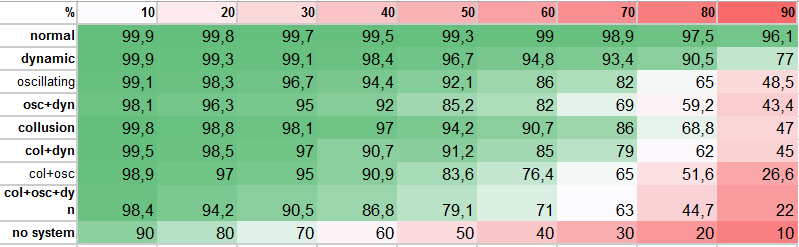
\includegraphics[scale={0.9}]
		{diagrams/table.PNG}
		\label{fig:table.PNG}
	\end{figure}
\begin{table}
\caption{Πίνακας μέσης ικανοποίησης}
\label{tab:avg_sat}
\end{table}

Εποπτικά μπορούμε να το δούμε τα ίδια συμπεράσματα και στο σχήμα \ref{fig:horizontal.PNG}
 
\diagram{Συμπεριφορά δικτύων}{horizontal.PNG}
\newpage
\section{Ταχύτητα σύγκλισης RT-IOT}

Σε αυτήν την ενότητα παρουσιάζεται πόσο γρήγορα (σε αριθμό συναλλαγών) η μέση ικανοποίηση των Εικονικών Οντοτήτων συγκλίνει στην τελική τιμή της. Για καλύτερη εποπτεία το πείραμα έγινε δύο φορές, την πρώτη το ποσοστό τον κακόβουλων οντοτήτων ήταν σε σχετικά φυσιολογικά επίπεδα (30\%), ενώ στο δεύτερο ήταν σε επίπεδα επίθεσης σε ολόκληρο το σύστημα (70\%). 

Παρακάτω είναι τα διαγράμματα και πάλι για διαφορά είδη δικτύων
\diagram{Ταχύτητα σύγκλισης σε δίκτυο με 30\% κακόβουλων οντοτήτων}{30.PNG}



Όπως μπορούμε να παρατηρήσουμε στο πρώτο σχήμα οι τιμές έχουν συγκλίνει από τους πρώτους 100 κύκλους επειδή σχεδόν όλοι βρίσκουν έναν ικανό αριθμό από καλόβουλες εικονικές οντότητες για να παίρνουν την υπηρεσία χωρίς να χρειαστεί να εξερευνήσουν πολύ. Ενδεικτικό είναι ότι από τους 10 πρώτους κύκλους η μέση ικανοποίηση είναι στο 90\% τις τελικής. Το ότι δεν φτάνουν όλα τα δίκτυα στο 100\% έχε να κάνει με το χρόνο που χρειάζονται οι εικονικές οντότητες να εντοπίσουν αλλαγή συμπεριφοράς και να βρουν κάποιον άλλον να πάρουν την υπηρεσία. 

Αντίθετα σε ένα απλό δυναμικό δίκτυο υπάρχει σύγκλιση στο 100\% επειδή στην λίστα φίλων είναι μόνο καλόβουλες εικονικές οντότητες οπότε μόλις βρεθεί κάποιος ανενεργός, ο επόμενος ενεργός εντός της λίστας θα δώσει την υπηρεσία καλά. Η χαμηλότερη ταχύτητα οφείλεται στο ότι πρέπει να συγκεντρώσει κάθε Ε.Ο. έναν αριθμό από φίλους το οποίο την κάνει αρχικά ευάλωτη σε επιθέσεις.

\diagram{Ταχύτητα σύγκλισης σε δίκτυο με 70\% κακόβουλων οντοτήτων}{70.PNG}
Στο δεύτερο σχήμα φαίνεται ότι η σύγκλιση θέλει παραπάνω κύκλους εκτός από την απλή περίπτωση. Αυτό συμβαίνει επειδή είναι δύσκολο να βρεθούν νέοι φίλοι αφού είναι πιθανό η πλατφόρμα να δίνει λάθος συστάσεις οπότε να χρειάζονται αρκετοί κύκλοι για να βρεθεί κάποιος καλός. 


Αυτό χειροτερεύει στην περίπτωση εναλλαγής συμπεριφοράς (osc) επειδή μπορεί μόλις εμπιστευτεί η Ε.Ο. κάποιον, αυτός να το εκμεταλλευτεί αλλάζοντας συμπεριφορά οπότε να χρειαστεί νέος κύκλος ερωτήσεων.
\newpage

\section{Σύγκριση με δημοφιλή συστήματα εμπιστοσύνης - φήμης}
Για να φανεί  πραγματική αξία του συστήματος σε αυτή την ενότητα
συγκρίνεται με τρία από τα επικρατέστερα συστήματα φήμης εμπιστοσύνης σήμερα (Eigentrust \cite{EigenTrust},PeerTrust\cite{PeerTrust},  PowerTrust\cite{PowerTrust}) 
 καθώς και με ένα σχετικά νέο συστήμα, γνωστό ως BTRM(Bio-Inspired Trust and Reputation Model\cite{BTRM})  εφαρμόζει έναν βιλογικό αλγόριθμο γνωστό ώς Ant-Colony System\cite{Dorigo} (ACS).



\subsection{Σύγκριση Μέσης Ικανοποίησης}

Διενεργήθηκαν πειράματα τόσο σε απλά δίκτυα όσο και σε δίκτυα με δυναμική είσοδο κόμβων ή εναλλαγή συμπεριφοράς. Έγιναν μετρήσεις για διάφορα ποσοστά κακόβουλων οντοτήτων (10,30,50,70,90).
\diagramscale{Σύγκριση σε απλό δίκτυο}{normalcmp.PNG}{0.9}
\diagramscale{Σύγκριση σε δίκτυο δυναμικής εισόδου κόμβων}{osccmp.PNG}{0.9}
\diagramscale{Σύγκριση σε δίκτυο δυναμικής συμπεριφοράς }{dyncmp.PNG}{0.9}
\newpage
Όπως φαίνεται λοιπόν από τα διαγράμματα το RT-IOT έχει συγκρίσιμες επιδόσεις ικανοποίησης σε όλα τα δίκτυα παρόλο που έχει σχεδιαστικούς περιορισμούς αφού οι Ε.Ο. δεν έχουν πλήρη εικόνα για την συμπεριφορά των υπολοίπων. Έτσι ο συνδυασμός κεντρικής αρχής και κατανεμημένων τρόπων υπολογισμού εμπιστοσύνης και φήμης οδηγεί σε ένα σύστημα ικανό να διατηρήσει την ικανοποίηση σε πολύ καλά επίπεδα.

\newpage
\subsection{Σύγκριση Κλιμάκωσης}

Όπως είδαμε το RT-IOT παρέχει παρόμοιες επιδόσεις με τα υπόλοιπα συστήματα σε όλους τους τομείς. Η διαφορά του όμως είναι στο σχεδιασμός από την αρχή. Ούτε η εικονικές οντότητες ούτε η πλατφόρμα έχουν πλήρη εικόνα του συστήματος κάτι που προσφέρει ένα τεράστιο πλεονέκτημα στην κλιμάκωση. Στο παρακάτω διάγραμμα φαίνεται πόσο κατάφεραν να κλιμακώσουν τα διάφορα συστήματα εμπιστοσύνης-φήμης στην προσομοίωση.

\diagramscale{Σύγκριση Κλιμάκωσης}{scale.PNG}{0.8}

Όλες οι μετρήσεις έγιναν σε προσωπικό υπολογιστή με Intel Core i7 3630QM και 8GB RAM. Δόθηκε όριο χρόνο 30sec ανά κύκλο συναλλαγών (1 βήμα στην προσομοίωση δηλαδή). Τα αποτελέσματα φαίνονται στο σχήμα \ref{fig:scale.PNG}. Σημειώνουμε πώς το RT-IOT δεν έφτασε τα 30sec/step αλλά μόνο τα 1 sec/step. Το πρόβλημα ήταν πώς δεν ήταν δυνατό να δημιουργηθούν άλλα threads στο σύστημα.

Όπως είναι εμφανές το RT-IOT κατάφερε να τρέξει προσομοίωση με δεκαπλάσιους κόμβους ενώ πιστεύουμε ότι με αρκετή μνήμη θα ήταν \textbf{250x} .

Γενικά παρατηρήθηκε σχεδόν σταθερός χρόνος/Ε.Ο. κάτι που μεταφράζεται σε σταθερό χρόνο ανά Ε.Ο. και γραμμική κλιμάκωση της πλατφόρμας.

\diagramscale{Χρόνος υπολογισμού βήματος ανά Ε.Ο στο RT-IOT}{timepernode.PNG}{0.8}

